% This file contains information on how to set up a Cassandra simulation
%
% Wrtten by Jindal Shah on 02/09/12
% Updated by Ed Maginn on 03/20/14
% Updated by Ed Maginn on July 27, 2014
\chapter{Cassandra Basics}
\section{Flow Diagram}
A flow diagram that overviews the setup for a Cassandra simulation is displayed on figure \ref{fig:flow_diagram}. 
This diagram employs two automation scripts located in the \texttt{/Scripts/} directory: \texttt{mcfgen.py} and \texttt{library\_setup.py}.
These scripts are particularly useful when simulating large molecules. 
For details about how to use them, please refer to sections \ref{sec:mcfgen} and \ref{sec:libgen} of this user guide, and to the README files located in 
the subdirectories inside the directory \texttt{/Scripts/}.

\begin{figure}[t]
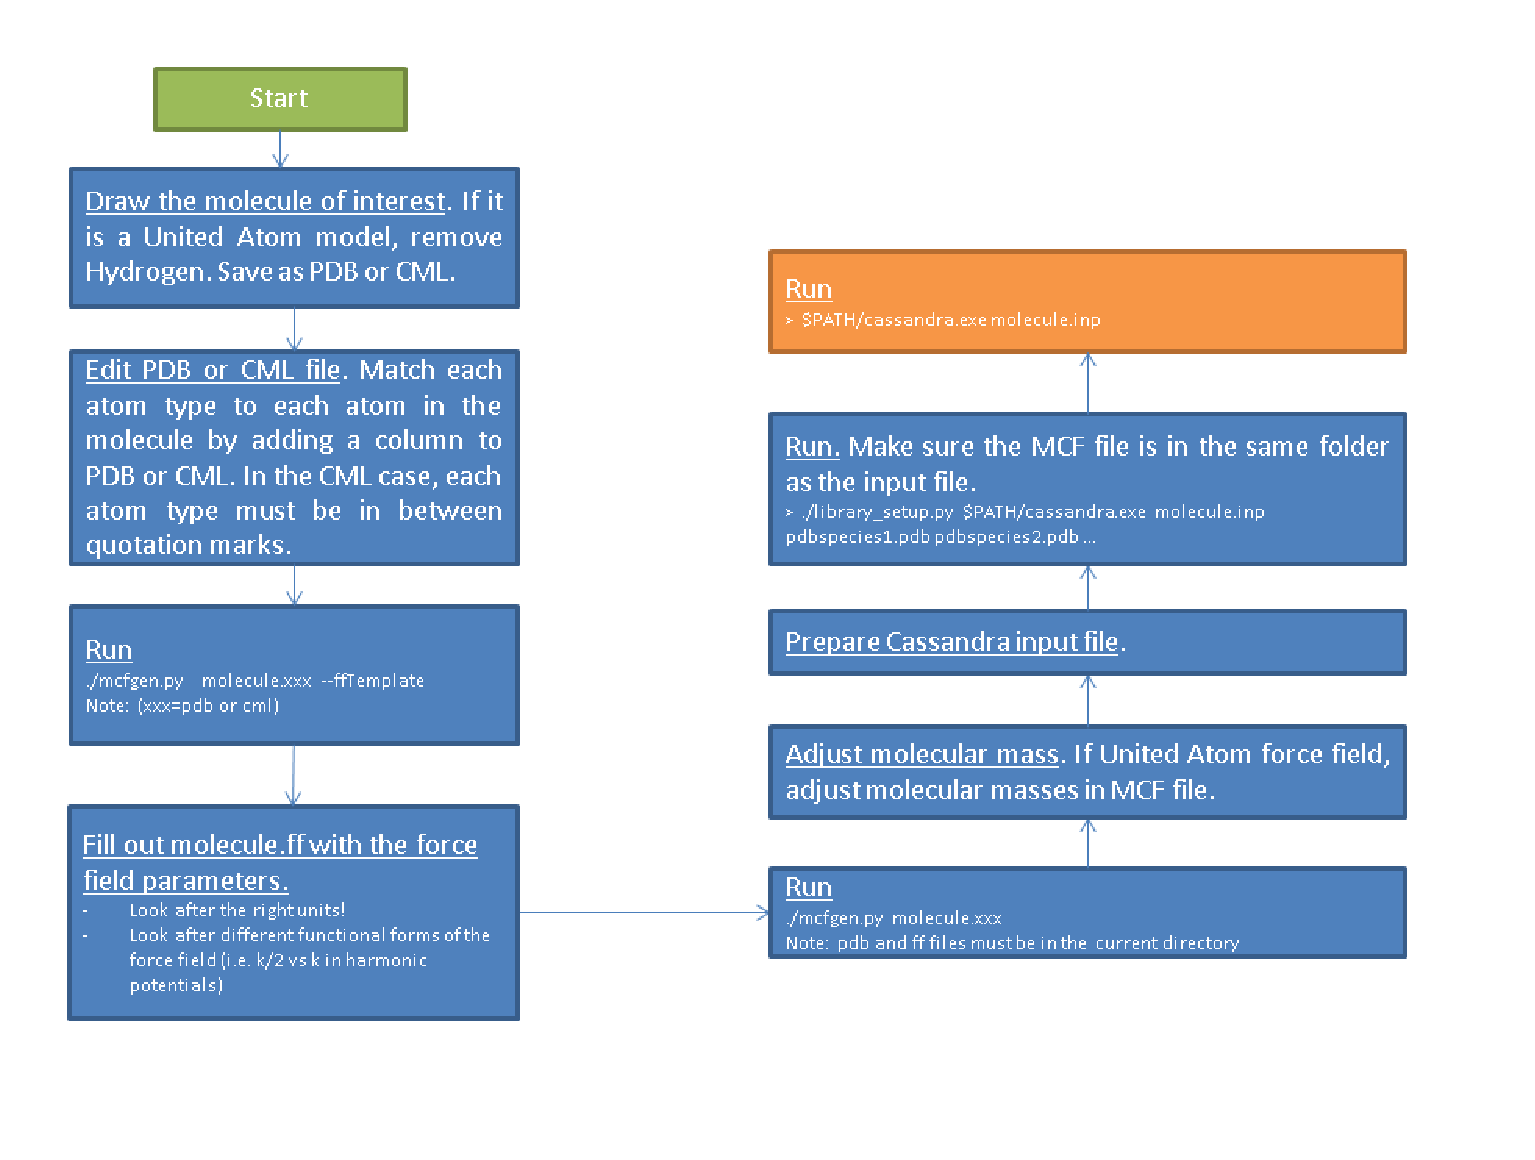
\includegraphics[width=\linewidth]{setup_flowdiagram.eps}
\caption{Flow diagram representing a typical setup of a Cassandra simulation}\label{fig:flow_diagram}
\end{figure}




\section{Cassandra Simulation Setup}

Once a system is identified, setting up a Cassandra simulation from
scratch requires preparation of the following files. \\

\begin{itemize}
\item A molecular connectivity file (MCF)  (*.mcf) containing the molecular
  connectivity information on bonds, angles, dihedrals, impropers and
  whether the molecule is composed of fragments. For information on
  the MCF file, please refer to section \ref{sec:MCF_File}.

\item An input file (*.inp) (see section \ref{sec:Input_File})

\item If the molecule is composed of fragments, then a fragment library file for each of the fragments is required. For instructions on how to generate these files, please refer to the
section \ref{sec:libgen}.

\end{itemize}
%
MCF files for united-atom models of methane, isobutane, dimethylhexane, cyclohexane and diethylether are provided in the \texttt{MCF} directory. Input files for NVT, NPT, GCMC and GEMC ensembles are located in the \texttt{Examples} directory which also contains fragment library files for a number of molecules simulated in these ensembles. 

%Examples of MCF, input files and fragment library files  can be found in the MCF and
%Examples directories repsectively. Fragment files are also located in the
%NVT - diethyether
%NPT - Water\_SPCE, Pentane, diethyether
%GCMC - Methane
%GEMC - Cyclohexane, Methane, Isobutane, Diethyether, Dimethylhexane

\section{Cassandra File Preparation}

\subsection{MCF File}
One MCF file is required for each unique species in a simulation. A
species is defined as a collection of atoms associated with each other
through bonds. Thus a molecule is a species as is an ion. If you
wanted to simulate sodium sulfate, you would need separate MCF files
for the sodium ion and the sulfate ion. MCF files can be created manually 
or by using the scripts provided with the code, as described in
the section \ref{sec:mcfgen}. Instructions for generating an MCF file can also be found in the \texttt{Scripts/MCF\_Generation/README} file. 
We will collect MCF files submitted to us by users and will post them on the Cassandra
website http://cassandra.nd.edu. If you have an MCF file you would
like us to post, send it to ed@nd.edu.
%
%
\subsection{Input File}
%
%
An input file is required for a Cassandra simulation. The input file
specifies conditions for the simulation and various keywords required
for the simulation in a given ensemble. Please refer to 
Chapter~\ref{sec:Input_File}  for further details.
%
\subsection{Fragment Library Generation}
Cassandra makes use of reservoir sampling schemes to correctly and efficiently sample the various coupled intramolecular degrees of freedom associated with
branch points and rings. For more information, please see Ref. \cite{Shah:2011}. 
The molecule is decomposed 
into fragments that are either branch points or ring groups,
each coupled to other fragments via a single dihedral angle. Thus, the
total number of fragments of a molecule is the sum of branch points
and ring groups in the molecule. The neighboring fragments are
connected by two common atoms present in each of the fragments. Note
that the ring group contains all the ring atoms and those directly
bonded to the ring atoms. For each fragment identified, Cassandra runs
a pre\textendash simulation in the gas phase to sample the intramolecular degrees
of freedom. A library of a large number of these conformations are
stored for use in an actual simulation. \\ \\
%
%
The gas phase library generation has been automated with the script \texttt{library\_setup.py} located in the \texttt{Scripts/Frag\_Library\_Setup}
directory. Use the following command for generating the fragment library. \\ \\
%
\texttt{> python \$PATH/Frag\_Library\_Setup/library\_setup.py \$PATH/Src/cassandra\_executable \\ input\_filename mol1.pdb (mol1.cml)  mol2.pdb (mol2.cml) ...}\\ \\
%
where \texttt{input\_filename} is the name of the input file for the actual simulation and \texttt{mol1.pdb mol2.pdb ...} or \texttt{mol1.cml mol2.cml ...} correspond to the
names of the pdb (or cml) files used to generated the MCF files. Make sure that if a file does not exist in the current working directory, its path relative
to the current working directory is specified. 

%If the molecule is not represented as a collection of fragments, then
%an initial configuration can be generated by simply supplying the name
%of the input file to the cassandra executable \\ \\
%%
%{\it \$cassandra\_path/cassandra.exe \$input\_file}.\\ \\
%%
%However, if the molecule is composed of fragments, two intermediate
%steps are required before a simulation is started: \\ 
%%
%\begin{itemize}
%\item Generation of mcf, xyz and car files for each fragment,
%\item Using the fragment mcf files to generate fragment conformations
%  at the temperature of the simulation. Thus, the fragment
%  conformations need to be regenerated if the simulation temperature
%  is changed.
%\end{itemize}
%
%\section{Cassandra Analysis}
%At present, Cassandra does not come with any analysis tools except a
%simple plotting script 'analysis.py'. The analysis script takes in the
%name of the input file as an argument. The analysis script will then
%figure out the number of properties specified in the input file and an
%xmgrace plot will be produced for each property as a function of Monte
%Carlo steps. Users should ensure that thermodynamic properties are
%converged for accurate average calculations.

\section{Running a Simulation}

To launch a Cassandra simulation, run the following command: \\ \\
%
\texttt{> cassandra\_executable input\_filename} \\ \\
%
The executable will read \texttt{input\_filename} and execute the instructions. Make sure that the required files (MCF, fragment library files) are located in the directories as given in the input file.

\section{Restarting a Simulation}
Restarting a simulation requires either a checkpoint file (*.chk produced
by Cassandra) or a configuration file obtained from xyz files generated
from a previous simulation. For the set up of these simulations, a script
in \texttt{Scripts/Read\_Old} is provided. Detailed instructions are contained
in the README file in this directory. 

%The 'checkpoint' option in the '\# Start\_Type' can be used to restart
%a simulation from a checkpoint file generated from a previous
%simulation. {\em An error in reading the checkpoint file
%  may occur if the '\# Sim\_Type' is not identical for both the simulations.'}
%
%When this option is used, the checkpoint file will be used
%to initialize the following variables.
%
%\begin{itemize}
%\item Total number of trials for displacement, rotation, dihedral and
%  angle moves for each species in every box.
%\item Total number of successful attempts for displacement, rotation,
%  dihedral and angle moves for each species in every box.
%\item Total number of successful volume moves and total number of
%  volume moves performed for each box in a simulation that involves
%  volume fluctuations.
%\item Total number of trials performed in each box.
%\end{itemize}
%
%The following variables will be {\em overwritten} by the checkpoint
%file. 
%
%\begin{itemize}
%\item Maximum displacement width, maximum rotational width and
%  torsional width for each species in every box.
%\item Box shapes
%\item Box lengths
%\item Maximum volume fluctuation for each box.
%\item Pore width and maximum change in pore width for a slit pore
%  simulation.
%\item Random number seeds.
%\end{itemize}
%
%\section{Restart Simulation - 'read\_config'}
%The 'read\_old' option in the '\# Start\_Type' can be used restart a
%simulation from an xyz file
%One input file is required for each box. The following procedure may be
%used to generated the last configuration file suitable for input to a
%Cassandra simulation.
%
%\begin{itemize}
%\item From the last output in the '\$input\_file\_Mov\_H.box*, extract
%  the information about the total volume, cell matrix,  number of
%  species and number of moles of each species in the box.
%\item From the last output in the '\$input\_file\_Mov\_XYZ.box*,
%  extract the last configuration.
%\item Open a new file named '\$input\_file.old.box*'.
%\item The first line will contain number of molecules of each species
%  in box*.
%\item Append the last configuration in the box obtained above.
%\end{itemize}
%
%
%
% Fragment generation
%
%
%
%\section{Fragment Generation}
%Cassandra uses an advanced configurational bias Monte Carlo scheme~\cite{Shah:2011,Macedonia:1999} for conformational sampling and insertion\/deletion of molecules. In this scheme, a molecule is decomposed into fragments and a conformational library, satisfying the bond angle probability distribution, for each of the fragments is generated in the gas-phase. The molecule is reconstructed by joining the fragments who conformations are chosen from these gas phase libraries. To carry out fragment-base simulation requires two steps: \\
%\begin{itemize}
%\item Generation of fragments for a given molecule.
%\item Generation of conformational library
%\end{itemize}
%%
%\subsection{Generation of fragments}
%This step is necessary to generate individual fragment MCF and CAR files that can be used for fragment library generation. For this step, a master MCF file of the parent molecule must be prepared. The '\# Sim\_Type' for this simulation is set to 'MCF\_Gen'. Note that, if there are ring atoms in the molecule, they must be explicitly identified in the master MCF file. {\bf At present, the code  identifies only non-ring fragments}. A sample input file is provided. At the successful completion of fragment generation, the user will see a number of files, such as {\em fragment\_1\_1.mcf, fragment\_1\_1.car} and corresponding xyz file and so on. Here the first index refers to the fragment while the second index refers to the species id.  For the generation of the CAR and XYZ files, the anchor atom is placed at the origin while other atoms are placed randomly on a sphere the radius of which is equal to the bondlength. 
%%
%If there are any rigid fragments in the molecule, the CAR and XYZ file coordinates generated at this step are not appropriate for actual simulations. See below.
%%
%\subsection{Generation of Fragment Library}
%%
%Once the MCF and CAR files are generated, an additional step of generating the conformational library for each of the unique fragments is carried out. Two fragments are considered identical if they contain same number of atoms; all the bond lengths are identical; the nominal values of all the bond angles are the same and so are the force constants.  For the library generation, an NVT Monte Carlo simulation is carried out with a single molecule in the gas phase. The '\# Sim\_Type' for such simulations are 'NVT\_MC\_Fragment' or 'NVT\_MC\_Ring\_Fragment' depending on whether a given fragment has cyclic fragments. Sample input files are provided for the user. In the non-ring fragment library generation, atom sampling algorithm is carried out to populate the fragment library. For ring fragment, flip move is performed in addition to the atom sampling for the library generation. Details of the algorithm can be found in Shah and Maginn~\cite{Shah:2011}.

\section{Cassandra Output Files}

Cassandra generates several output files which can be used for later analysis. All have as a prefix the Run\_Name specified in the input file. See Chapter \ref{sec:Input_File} for details. The type of output is specified by the file name suffix. The following are generated:

\begin{itemize}

\item {\bf Log file} (*.log): Contains basic information on what the run is, timing information and reports the various parameters specified by the user. A complete copy of the input file is reproduced. Other important information includes the move acceptance rates. You can use the log file to keep track of what conditions were simulated.

\item {\bf Coordinate file} (*.xyz or *.box\#.xyz): For each box in the system, a set of xyz coordinates are written out with a frequency specified by the user (Coord\_Freq). The file has as a header the number of atoms in the box. Following this, the atomic coordinates of molecule 1 of species 1 are written, then the coordinates of molecule 2 of species 1 are written, etc. After all the coordinates of the molecules of species 1 are written, the coordinates of the molecules of species 2 are written, etc. You can use this file to do all your structural analysis and post processing.\\

Note that if you generate your initial configuration using the make\_config command, the first ``snapshot'' of the coordinate file
will contain the initial configuration of all the species in the system for a given box. You can use this configuration to check on whether the initial configuration 
is reasonable, or use it as an input to other codes. Note that the initial configuration will be generated using a configurational biased scheme,  
so it may be a better starting configuration than if you used other methods. 

\item {\bf Checkpoint file} (*.chk): A checkpoint file is written every Coord\_Freq steps. This can be used to restart a simulation from this point using all of the same information as the run that was used to generate the checkpoint file. To do this, you must use the checkpoint restart option (see Chapter \ref{sec:Input_File}). It will basically pick up where the simulation left off, using the same random number seed, maximum displacements, etc. This is useful in case your job crashes and you want to continue running a job. You can also use the checkpoint file to start a new simulation using the  configuration of the checkpoint file as an initial configuration and the optimized maximum displacements.  To do this, use the script read\_old.py. You will need to set a new random number seed if you do this. See the documentation in Chapter \ref{sec:Input_File} for more details.

\item {\bf H-matrix file} (*.H or *.box\#.H): This file is written to every Coord\_Freq MC steps. The first line is the box volume in angstrom$^3$. The next three lines are the box coordinates in angstrom in an H-matrix form. Since Cassandra only supports cubic boxes at the moment, this is just a diagonal and symmetric matrix, but is included here for later versions that will enable non-orthogonal boxes. After this, a blank line is written. The next line is the box number, and the final line(s) is(are) the species ID and number of molecules for that species in this box. If there are three species, there will be three lines. This output is repeated every Coord\_Freq times. This file allows you to compute the density of the box during constant pressure simulations.  


\item{{\bf Property file}} (*.prp\# or *.box\#.prp\#): This file lists the instantaneous thermodynamic and state properties for each box. Note that you can have more than one property file (hence the\# after `prp') and more than one box (also why there is a \# after `box'). The user specifies which properties are to be written and in what order, and these are then reproduced in this file. The file is written to every Prop\_Freq steps. A header is written to the first two lines to designate what each property is. You may use this file to compute thermodynamic averages.

\end{itemize}
